\chapter{Descrição do problema}\label{chapter:description}

O desenvolvimento de uma plataforma colaborativa apresenta diversos desafios ao nível da sua arquitetura, 
do modelo de dados a construir e das decisões de implementação ao longo do seu desenvolvimento. 
Neste capítulo irá ser abordado as decisões tomadas no desenvolvimento do projeto, tendo em conta a plataforma \textit{OutSystems}. 
Irá ser feita uma descrição mais detalhada da solução adotada, acompanhada por um diagrama de blocos, que permite esquematizar a mesma.


\section{Diagrama de blocos da solução}\label{sec:diagram}
A figura~\ref{fig:diagram} apresenta o diagrama de blocos da solução. 

\begin{figure}[H]
  \centering
  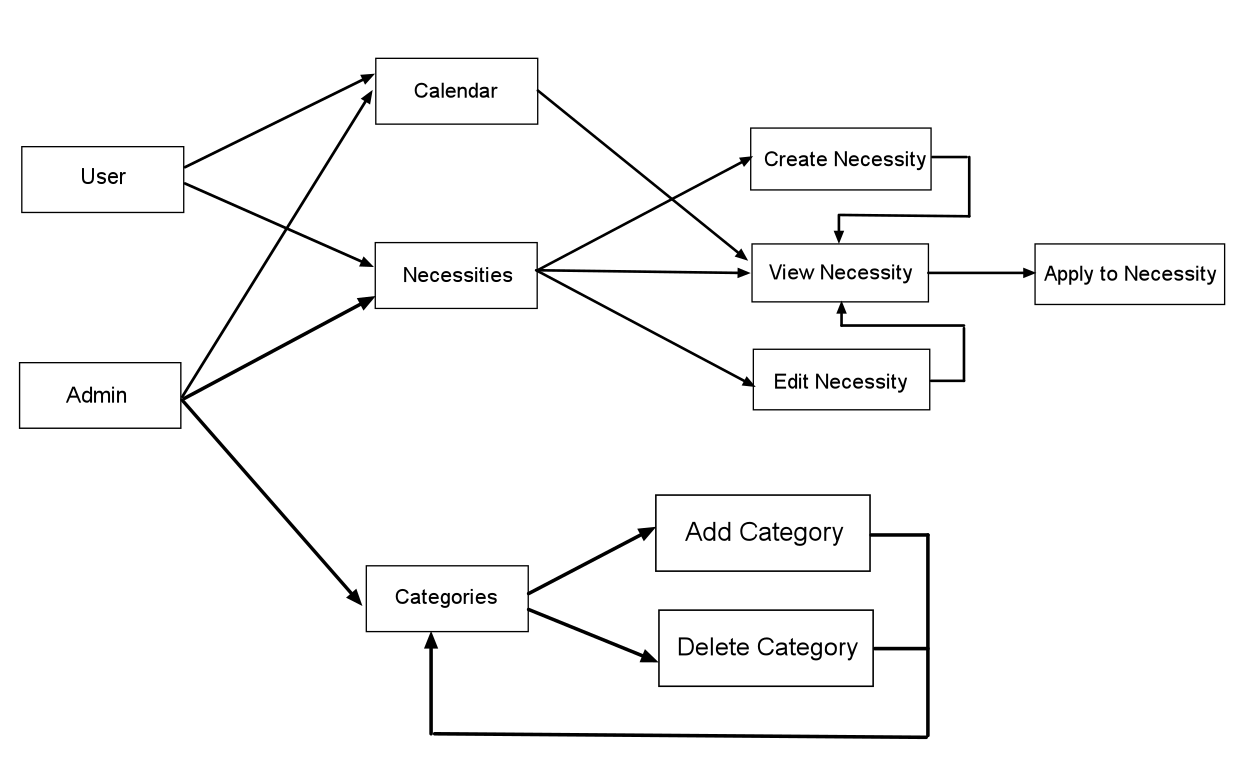
\includegraphics[scale=0.4]{figures/Diagrama de blocos.png}
  \caption{Diagrama de blocos da aplicação}\label{fig:diagram}
\end{figure}

\newpage

\section{Arquitetura}\label{sec:arquitechture}

\subsection{Plataforma \textit{OutSystems}}

A arquitetura desta plataforma pode ser observada na figura~\ref{fig:outsystemsArch}. 
O principal componente da plataforma é o Platform Server que permite que as aplicações 
desenvolvidas sejam geradas, optimizadas, compiladas e publicadas. 

\begin{figure}[H]
  \centering
  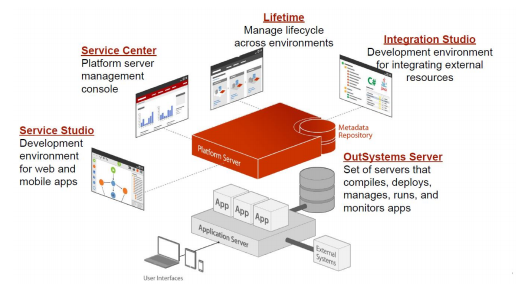
\includegraphics[]{figures/Architecture.png}
  \caption{Arquitetura da plataforma \textit{OutSystems}}\label{fig:outsystemsArch}
\end{figure}

Este componente usa os seguintes serviços: 
\begin{enumerate}
  \item \textit{Code Generator} --- Usa a aplicação modelada no \textit{Service Studio} e gera o código necessário usando tecnologias standard (como \textit{.NET, SQL Server, HTML,} etc.) para a criação de uma aplicação optimizada e segura.
  \item \textit{Deployment Services} --- Publica o código que foi previamente gerado no servidor, assegurando que a aplicação é instalada consistentemente em cada front-end da infraestrutura.
  \item \textit{Application Services} --- Gere as aplicações durante o runtime, através da execução de \textit{batches} agendados e serviços de \textit{logging} assíncronos que permitem que sejam armazenados eventos como erros, inspeções e métricas de desempenho.
\end{enumerate}

\newpage

\subsection{Arquitetura 4 Layer Canvas}\label{sec:4lc}

Para desenharmos a arquitetura da nossa solução, seguimos a metodologia da plataforma \textit{OutSystems}, a \textit{4 Layer Canvas}.

\begin{figure}[H]
  \centering 
  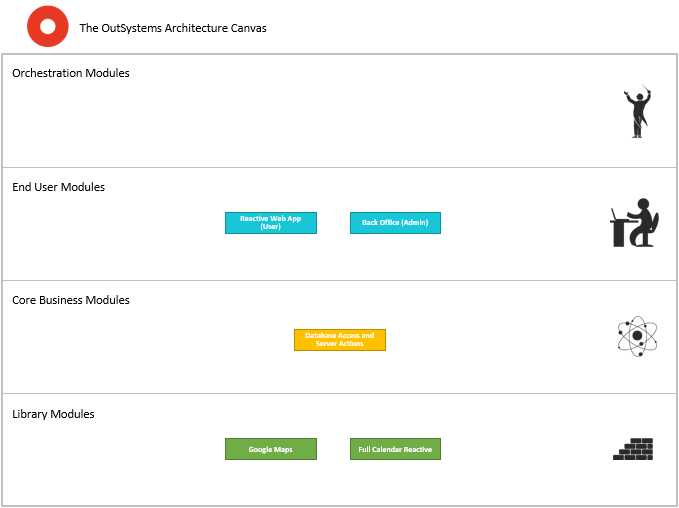
\includegraphics[scale=0.7]{figures/4LayerCanvas.png}
  \caption{4 \textit{Layer Canvas}}\label{fig:4lc}
\end{figure}

Esta metodologia propõe que se estruture as várias funcionalidades da aplicação por quatro camadas, sendo estas, começando por baixo: 

\begin{itemize}
    \item \textit{Library Layer} --- Aqui devem constar os módulos que são transversais ao domínio do problema, tais como: temas, bibliotecas, etc. 
    \item \textit{Core Layer} --- Módulos referentes à lógica de negócio, modelo de dados e \textit{server actions}. 
    \item \textit{End User Layer} --- Nesta camada é tratada toda a parte de interface e experiência do utilizador, fazendo uso das camadas anteriores. 
    \item \textit{Orchestration Layer} --- Camada que coordena a comunicação entre várias aplicações. 
\end{itemize}

É importante verificar que, apesar da metodologia apresentar quatro camadas, 
a nossa arquitetura apenas faz uso das primeiras três devido ao nosso projeto consistir em apenas uma aplicação reactive, 
e não havendo necessidade de coordenar interações com outras aplicações na camada de orquestração. 
Posto isto, a nossa aplicação assenta sobre cinco módulos, representados pela figura~\ref{fig:4lc}.

Começando pela \textit{Library Layer} verificamos que são utilizados os módulos relativos à integração da aplicação 
com o \textit{Google Maps} e com o \textit{Full Calendar Reactive}. De seguida temos a \textit{ Core Layer}, 
onde definimos as entidades de domínio e suas operações. Por fim a \textit{ End User Layer} onde são definidos 
os ecrãs e a lógica de cliente. 

\section{Modelo de Dados}\label{subsec:ModeloDados}

O conceito predominante no modelo de dados, (figura~\ref{fig:modeloDados}), é o de necessidade, representado pela tabela \textit{Necessity}.

\begin{figure}[H]
  \centering 
  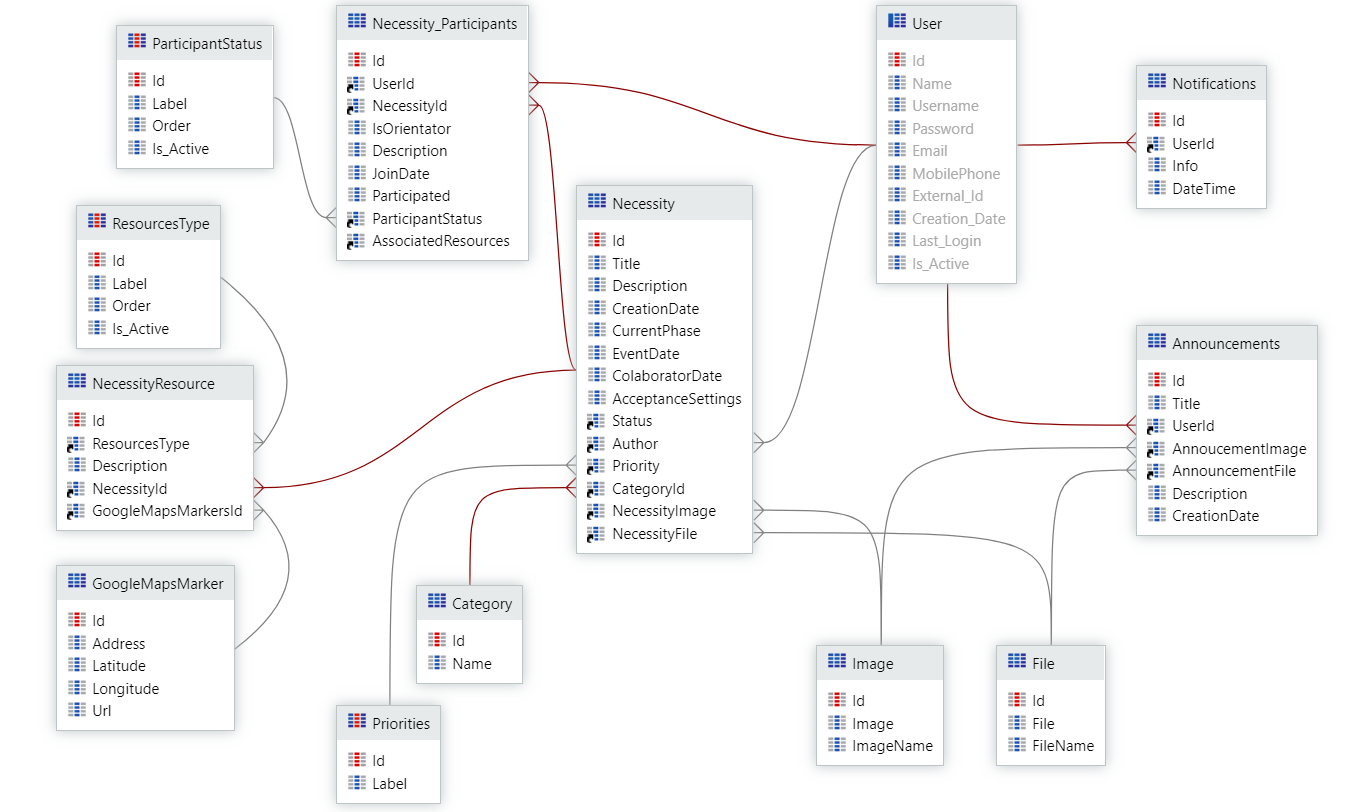
\includegraphics[scale=0.4]{figures/DataModel.png}
  \caption{Modelo de dados}\label{fig:modeloDados}
\end{figure}

 
Uma necessidade é caracterizada por diversos elementos dos quais destacamos o \textit{Status} que referencia uma tabela estática (\textit{NecessityStatus}) que contém os valores possíveis do estado da necessidade, 
podendo ter os valores \"Closed\", \"Active\" ou \"Archived\". A \textit{CurrentPhase} que indica a fase de candidaturas atual, 
podendo ser para orientadores ou participantes, a \textit{ColaboratorDate} que representa a data limite das candidaturas 
à posição de orientador e ainda \textit{AcceptanceSettings} que indica se para a necessidade em causa são aceites todos os participantes ou se existe uma filtragem por parte do autor. 
As tabelas \textit{NecessityImage} e \textit{NecessityFile} existem para o propósito de guardar ficheiros, 
aliviando a quantidade de dados guardada em cada tuplo \textit{Necessity}, 
seguindo também as boas práticas da plataforma \textit{OutSystems}. 
A entidade estática \textit{Priorities} contém os valores possíveis das prioridades que cada necessidade pode ter.
Associado ao conceito de necessidade está o de recurso, que tem como objetivo acrescentar informação à necessidade de uma forma flexível. Para suportar este conceito foi definida a entidade estática \textit{ResourcesType} cujos valores representam os tipos de recursos que um utilizador pode, facultativamente, acrescentar à necessidade, consistindo em acomodação, restaurante e menus de refeições, localização do evento ou transporte. A representação de um recurso no modelo de dados traduz-se na entidade \textit{NecessityResource} que guarda informações de cada recurso como o seu tipo (referência à tabela  \textit{ResourcesType}), a sua descrição, o id da necessidade a que o mesmo pertence e, como todos os recursos à exceção do relativo ao transporte têm um mapa do \textit{Google Maps} associado, o último atributo da tabela \textit{NecessityResource} é um id do marcador do mapa associado ao recurso.
Com o objetivo de guardar informação sobre os participantes de uma necessidade, é definida a entidade \texttt{\textit{Necessity\char`_Participants}} que 
contempla o identificador da mesma, o identificador do utilizador, a descrição associada à candidatura, 
se esta candidatura é para posição de orientador ou de participante, a data da candidatura, se o utilizador participou na necessidade, qual o estado da candidatura e os recursos associados a este participante. 
Um utilizador pode ser um participante, um autor ou um orientador da necessidade. 
Os comunicados feitos na plataforma são suportados pela entidade \textit{Announcements}. As notificações apresentadas na plataforma são suportadas pela entidade \textit{Notifications} em que cada notificação está associada a um utilizador através do seu id, o seu conteúdo é guardado no atributo \textit{Info} e a hora da emissão da notificação no atributo \textit{DateTime}. 
Um utilizador pode ainda ter o cargo de administrador, cujos privilégios incluem editar as categorias representadas pela entidade \textit{Category}.

\section{Implementação}\label{sec:implementacao}

\subsection{Autenticação}\label{subsec:implementacao:login}

Para realizar a autenticação de um utilizador, este introduz as suas credenciais nos respetivos \textit{input fields} e clica no botão \textit{Login}.
Se as credenciais introduzidas não corresponderem às de nenhum utilizador na base de dados, será apresentada uma mensagem de erro.
Um utilizador só terá acesso a outros ecrãs se tiver autenticado, caso contrário será redirecionado para este ecrã.

\subsection{Dashboard}\label{subsec:implementacao:dashboard}
%LEMBRAR PARA METER AS NECESSIDADES ATIVAS NA PARTE DAS PRIORIDADES
Este é o ecrã apresentado a um utilizador autenticado assim que abre a aplicação.
O mesmo apresenta quatro \textit{widgets} que apresentam informação sobre o número de utilizadores que estão \textit{logged in} e o número de necessidades abertas com as suas respetivas prioridades (\textit{high, medium, low}).
Este ecrã apresenta também um gráfico com informação sobre as categorias existentes e a distribuição do número de necessidades criadas em cada uma das mesmas.
A seleção de uma categoria do gráfico promove a navegação para o ecrã das necessidades,  apresentando a lista das mesmas que pertencem à categoria selecionada.
Para cada uma das prioridades que as necessidades podem ter, é apresentado um \textit{ranking} dos utilizadores que mais criaram necessidades, com a respetiva prioridade.

\subsection{Visualização de necessidades}\label{subsec:implementacao:necessities}
%WHEN CSS IS DONE PUT A NICE PICTURE HERE :D
O utilizador ao carregar no botão \textit{Necessities} presente na barra da aplicação, será redirecionado para o ecrã responsável pela apresentação das necessidades. 
O intuito do mesmo consiste na apresentação das necessidades criadas pela comunidade empresarial, sendo possível aplicar filtros e/ou pesquisar pelo título de uma necessidade de modo a que sejam apresentadas apenas as necessidades alvo.
As necessidades são apresentadas num \textit{widget} tabela, cujas colunas apresentam informação relevante como título, categoria, prioridade, estado, data de criação e data em que a necessidade irá decorrer. Sempre que o utilizador pretender criar uma nova necessidade, apenas tem que carregar no botão \textit{Create Necessity} e será redirecionado para um novo ecrã, onde poderá completar a criação.
A seleção do título de uma necessidade promove a navegação para o ecrã dos detalhes da mesma.
A barra de pesquisa permite que o utilizador procure uma necessidade pelo seu título.
Os filtros aplicáveis são apresentados em dois \textit{dropdowns}, um para permitir a escolha de qual a prioridade e outro para seleção da(s) categoria(s).
Sempre que exista uma mudança na seleção de algum dos \textit{widgets} de filtragem de necessidades ou uma introdução de texto na barra de pesquisa, a tabela é atualizada para apresentar apenas aquelas que verifiquem as características alvo. 
As informações de cada uma das necessidades, das categorias existentes e das prioridades são obtidas comunicando com o servidor através de \textit{Aggregates}. 
Estes \textit{Aggregates} são \textit{querys} optimizadas à base de dados de modo a retornar informação de forma eficiente e apresentá-la nos \textit{widgets} do ecrã.


\subsection{Visualização de necessidades num calendário}\label{subsec:implementacao:calendarNecessitiesView}
%WHEN CSS IS DONE PUT A NICE PICTURE HERE :D
O utilizador ao carregar no botão \textit{Calendar} presente na barra da aplicação, será redirecionado para o ecrã responsável por mostrar, num calendário, todas as necessidades existentes organizadas por datas. 
O objetivo deste ecrã é apresentar de uma forma mais organizada e estruturada todas as necessidades criadas pela empresa, sendo possível filtrá-las. 
Para preencher o calendário, para cada necessidade, é criado um objeto \textit{Event} com a sua informação. 
Cada evento estará representado no calendário com uma cor diferente de forma a distinguir entre necessidades criadas pelo utilizador, necessidades associadas, nomeadamente uma inscrição, e necessidades criadas por outros utlizadores.
Se o utilizador carregar num evento, este é redirecionado para o seu ecrã de detalhe. 
É possível filtrar eventos pela sua categoria, através de um popover menu que contém todas as categorias existentes. 
Caso seja selecionada uma categoria, são removidos todos os eventos presentes no calendário, e de seguida, renderizado com os novos eventos filtrados.


\subsection{Criação e edição de necessidades}\label{subsec:implementacao:necessityCreation}

O ecrã \textit{NecessityCreation} é utilizado para criar, editar, remover ou ver os detalhes de uma necessidade.
No momento da criação de uma necessidade os \textit{widgets} presentes neste ecrã permitem que o utilizador indique o título, a descrição, a categoria a qual associar a necessidade, a sua prioridade, 
se existe filtragem de participantes ou todas as candidaturas são aceites, uma imagem e um ficheiro para serem associados à necessidade, a data em que a mesma irá decorrer, se é necessário colaborador(es) e a data limite para a(s) sua(s) candidatura(s).

Ao pressionar o botão presente no final do ecrã com a legenda \textit{Save}, tanto num cenário de edição como de criação, 
são guardadas as informações presentes nos \textit{widgets} e é desencadeada uma \textit{client action} que posteriormente cria uma ligação ao servidor através da chamada a uma \textit{server action} para modificar a base de dados com uma nova necessidade ou alterando uma necessidade pré-existente.

Se o utilizador desejar editar ou remover uma necessidade, só o poderá fazer se for o autor desta e, no caso de a editar, o ecrã apresentará os campos já preenchidos com os dados atuais da necessidade e a possibilidade de os alterar livremente.
É também neste ecrã que o utilizador poderá consultar os recursos associados através da navegação até à tab \textit{Resources} e se for o autor da necessidade pode adicionar novos recursos. 
Todos os recursos com exceção do recurso transporte têm um \textit{block} que contém um mapa do \textit{Google Maps} através do qual o utilizador pode colocar um marker para dar a conhecer a localização associada ao recurso. 
A integração do \textit{Google Maps} na plataforma é realizada através da comunicação com a API do \textit{Google Maps}. Para criar um novo mapa é necessário criar um objeto do tipo \textit{google.maps.Map} que recebe na sua construção o elemento html onde o mapa será inserido. 
Toda a dinâmica de interação com o mapa é gerida pela API através de eventos que são desencadeados com o toque no mesmo. 

Na última tab do \textit{widget Accordion} presente no ecrã \textit{NecessityCreation} encontra-se a secção relacionada com os participantes à necessidade. 
Nesta secção um utilizador poderá candidatar-se à posição de colaborador ou participante, de acordo com a fase em que a necessidade se encontra, carregando no \textit{widget link} com o texto \textit{Apply as a Colaborator/Partipant} e deixando uma descrição se a filtragem dos candidatos estiver ativa para aquela necessidade.
Um utilizador, ao criar uma necessidade, tem a opção de escolher se todas as candidaturas são aceites ou se o próprio irá proceder à sua filtragem selecionando um dos \textit{widgets radio button}.  